\section{Image Segmentation}
\tocless\subsection{Fully Convolutional Neural Networks for Semantic Segmentation}
There has been a very interesting paper from UC Berkeley focused on using Full Convolutional
Networks for semantic segmentation \parencite{fcn}. Fully Convolutional Networks
(FCN)
do not have any fully connected layers. They are replaced with more filtering
layers. Nvidia Digits have a semantic segmentation implementation based off the
work of this paper.

They took this approach because "feedforward computation and backpropogation are
much more efficient when computer layer-by-layer over an entire image instead of
independently patch-by-patch" \parencite{fcn}. This was also because they
were focused on object detection. Normal classifiers do not work very well when
they are to classify more than one subject in an image and image segmentation
was a way to solve this.

There are a set of steps you can follow to turn a CNN into a FCN for semantic
segmentation as follows ie. change to a convolutional layer from a fully
connected one:
\begin{itemize}
    \item{The size of the filters must be set to the size of the input layers.}
    \item{For every neuron in the fully connected layer, have a filter.}
\end{itemize}

\begin{table}[]
\centering
\caption{FCN Resulys \parencite{fcn}}
\label{fcn}
\begin{tabular}{ll}
                        & FCN  \\
VOC11 mean IU           & 62.7 \\
VOC12 mean IU           & 62.2 \\
PASCAL VOC10 pixel acc. & 67.0 \\
PASCAL VOC10 mean acc.  & 50.7 \\
PASCAL VOC10 mean IU    & 37.8 \\
PASCAL VOC10 f.w. IU    & 52.5
\end{tabular}
\end{table}

\tocless\subsection{Segmentation}
\subsubsection*{Graph Based Segmentation}
Graph cut segmentation has been used extensively  in image segmentation. OpenCV
has an implementation of a graph cut algorithm called grabcut which has been
used to segment food on occasion \textcite{graphCut}. 

According to \textcite{graphCut}, "Graph cut based method is well-known to be
efficient, robust, and capable of finding the best contour of objects in n
image, suggesting it to be a good method for separating food portions in a food
image for calorie measurement". Along with the graph cut segmentation algorithm,
this research team also used color and texture segmentation. Gabor filters were
used to measure texture features \textcite{graphCut}. When color and texture
segmentation was applied, the method came into difficulty with mixed foods but
by applying graph cut segmentation, clearer object boundaries were shown.

In conclusion, the accuracy of the classification increased when using graph
based segmentation rather than color and texture as seen in \ref{graphCT}.

\begin{table}[]
	\centering
	\caption{Results}
	\label{graphCT}
	\begin{tabular}{llll}
		                  & Single Food Portion & Non-mixed Food & Mixed Food
						  \\
						  Color and Texture & 92.21               & N/A
						  & N/A           \\
						  Graph Based       & 95 (3\% increase)   & 5\% increase
						  & 15\% increase
	\end{tabular}
\end{table}

\subsubsection*{Local Variation Framework}
Another paper was published in which the research team attempted to create a
food calorie extimation system \textcite{foodImageAnalysis}. This system would
compromise of three steps, image segmentation, image classification and weight
estimation. For the segmentation module, a local variation approach to
segmentation was performed. Local variation is by which intensity differences
between neighbouring pixels is measured. This is a type of graph based
segmentation.

The team also carried out some segmentation refinement when the segmentation
algorithm had been performed. This consisted of removed small segments (defined
as less than 50 pixels) and trying to prevent over and under segmentation. After
classification was performed on each segment, segments with low confidence
values were removed \textcite{foodImageAnalysis}.

\subsubsection*{Conclusion}
Both of the above papers of \textcite{graphCut} and \textcite{foodImageAnalysis}
used a graph based segmentation. The first paper used a more generic
implementation while the second used a local variation framework. Both methods
provided successful results in the image segmentation process.


% \begin{figure}
%     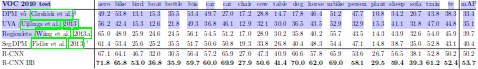
\includegraphics[width=150mm,scale=0.5]{DAP}
%     \caption{Detection Average Precision \parencite{donahue}}
%     \label{fig:dap}
% \end{figure}

% \begin{figure}
%     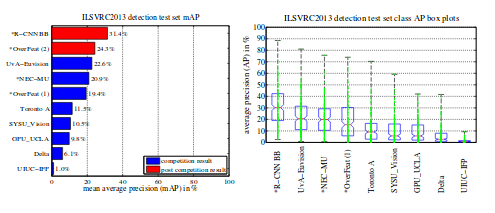
\includegraphics[width=150mm,scale=0.5]{MAP}
%     \caption{Mean Average Precision \parencite{donahue}}
%     \label{fig:MAP}
% \end{figure}

% \begin{figure}
%     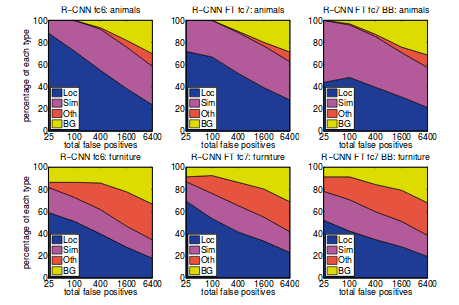
\includegraphics[width=150mm,scale=0.5]{DFP}
%     \caption{Distribution of top-ranked false positives
%     \parencite{donahue}}
%     \label{fig:DFP}
% \end{figure}

% \begin{figure}
%     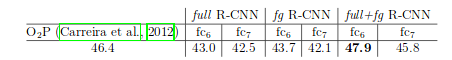
\includegraphics[width=150mm,scale=0.5]{SMP}
%     \caption{Segmentation Mean Accuracy \parencite{donahue}}
%     \label{fig:SMP}
% \end{figure}

% \begin{figure}
%     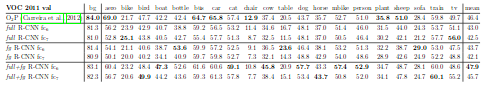
\includegraphics[width=150mm,scale=0.5]{PCATSA}
%     \caption{Per-category segmentation accuracy \parencite{donahue}}
%     \label{fig:PCATSA}
% \end{figure}

% \begin{figure}
%     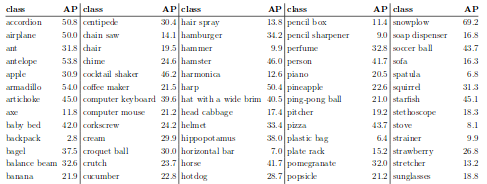
\includegraphics[width=150mm,scale=0.5]{PCLASSSA}
%     \caption{Per-class segmentation accuracy \parencite{donahue}}
%     \label{fig:PCLASSA}
% \end{figure}

% \begin{table}[]
%     \centering
%     \caption{Project Plan}
%     \label{pp}
%     \begin{tabular}{ll}
%         Task/Deliverable                     & Deadline \\
%         Interim Report                       & 21/12/17 \\
%         Select method and paper to replicate & 10/01/18 \\
%         Iteration 1                          & ???      \\
%         Iteration 2                          & ???      \\
%         Iteration 3                          & ???      \\
%         Draft Final Report                   & 08/03/18 \\
%         FYP Product                          & 10/04/18 \\
%         FYP Report                           & 17/04/18
%     \end{tabular}
% \end{table}
